\documentclass[a4paper]{article}
\usepackage[utf8]{inputenc}
\usepackage[english]{babel}
\usepackage{moreverb}
\usepackage{graphicx}
\usepackage{fancyvrb}
\usepackage{float}
\title{Project Report \\ \emph{Krusty Kookies Sweden AB} \\ EDA216 Database Technology}
\date{\today}
\author{Fredrik Paulsson \\ D11 \\ dat11fp1@student.lu.se \and Jonas Jacobsson \\ D11 \\ dat11jja@student.lu.se}
%\setcounter{secnumdepth}{5}
%\setcounter{tocdepth}{5}
\begin{document}
\maketitle
%\tableofcontents
\newpage

%Report
%The report should be written in English (you may write in Swedish if you absolutely cannot produce readable English). Contents:
%2
%1. A cover sheet with the name of the project, your names, education programs, and e-mail addresses. You must check mail to these addresses regularly.
%Also give the date of submission and complete instructions for running your program.
%2. An introduction (what the project is about, etc.).
%3. Something about requirements that you fulfill or don’t fulfill.
%4. An outline of your system (which database manager you use, which programs you have
%written, how the programs communicate with the database, etc.).
%5. An E/R diagram which describes the system.
%6. Relations. Indicate primary keys, possibly secondary keys, and foreign keys. You must
%show that the relations are normalized according to your chosen normal form (if a relation “obviously” is in BCNF you may say so, provided that you justify your statement). If a
%relation is in a lower normal form than BCNF, you must justify this choice.
%7. SQL statements to create all tables, views, stored procedures, and other database elements.
%(Don’t include statements to create the initial contents of the database.)
%8. A user’s manual (not necessary if everything in the program is self-explanatory).

\section{Introduction}
In this project we were to develop a database system that handles production, orders and deliveries of cookies in the company Krusty Kookies Sweden AB. In order to develop the database system we have to produce an E/R model of the database, create relations corresponding to the E/R model and finally implement those relations in a database management system. In the project we also had to implement a client program that interfaces to our database. This client program only handles production of cookies and blocking of pallets.

This report serves as documentation of our implementation. 

\section{Requirements}
Our database system can handle everything from ingrediences in the recipes to delivery of the cookies. 

When a new pallet is created the stock of the ingredients to make the recipe are updated to make sure the quantities of the ingredients in stock are correct. It is possible to create several pallets of a given cookie at the same time.

The pallets are registered in our database when entering the freezer. However in this pilot implementation the pallets are assumed to be in the freezer immediately after they have been produced. To identify every pallet each pallet has a unique ID.

We can show all kinds of information that is relevant about pallets through our search function. With this you can search for pallets by entering either pallet ID, recipe or the time when the pallet was produced.

If a batch of cookies do not meet the quality standards, you are able to block the pallets that are affected. Either through the pallet id or through the time which the batch was made. 

The database also handles customers and orders, each order has a unique ID to be able to easily identify them. The database also contains information about which pallets that are delivered and these pallets are associated to an order. For each order there exist information about the amount of pallets of different recipes that are to be delivered. However our database does not include a constraint that if delivered pallets associated with an order actually contains the correct type of cookies to be delivered or the amount of pallets to be delivered. We have assumed that is done either manually at the factory or by the client program that interfaces to the database and handles orders and deliveries.

The only client interface that we have developed are the one handling production, searching and blocking of pallets.



% Du kan fylla på lite om order och production. CHECK/Fredrik

\section{System Outline}
Our system uses MySQL as the database management system and our client interface is written in PHP for optimal portability. In PHP we have used PHP Data Object to interface with the MySQL server.

The following files make up the client part of our solution:


\begin{description}
\item[\texttt{index.php}] This is the home page of our implementation. This file also intiates communication with the database for the session.
\item[\texttt{cannotConnect.html}] This is simply an HTML file which is displayed if a connection the databse cannot be made.
\item[\texttt{mysql\_connect\_data.inc}] This file contains the login credentials to access the database.
\item[\texttt{database.inc.php}] This file contains all operations that are made to the database. Every other file uses this class to access the database.
\item[\texttt{produce1.php}] This file prompts the user for a recipe and amount of pallets to produce of that recipe.
\item[\texttt{produce2.php}] This file produces the pallets chosen in \texttt{produce1.php} and displays their ID:s.
\item[\texttt{sob1.php}] This file contains links to the search and unblock interfaces and the forms used to block/unblock pallets.
\item[\texttt{sob1search.php}] This file contains the forms used to search for pallets. 
\item[\texttt{sob1SearchResultID.php}] This file searches for the pallets and displays the results.
\item[\texttt{sob1betweenDates.php}] This file blocks/unblocks pallets that are made between given dates.
\item[\texttt{sob1blockedID.php}] This file shows the blocked pallets and also presents the user with the option of unblocking these pallets.
\end{description}
\section{E/R Model}
The UML diagram that displays our E/R model is shown in figure \ref{uml}.

\begin{figure}[t]
\centering
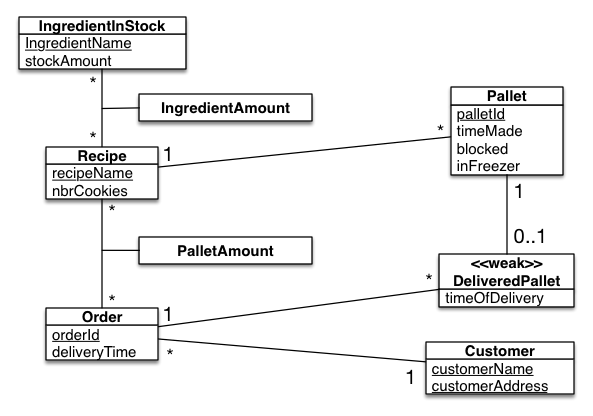
\includegraphics[scale=0.7]{projectUMLFinal.png}
\caption{UML diagram for the E/R model.}
\label{uml}
\end{figure}

\section{Relations}
The relations that we have produced from our E/R model is follows:

\vspace{0.5cm}

\noindent \texttt{IngredientsInStock(\underline{ingredientName},stockAmount)} \\
\texttt{Recipes(\underline{recipeName},nbrCookies)} \\
\texttt{IngredientsInRecipe(\underline{\textit{ingredientName},\textit{recipeName}},ingredientAmount)} \\
\texttt{Customers(\underline{customerName,customerAddress})} \\
\texttt{Orders(\underline{orderId},deliveryTime,\textit{customerName,customerAddress})} \\
\texttt{RecipesInOrders(\underline{\textit{recipeName},\textit{orderId}},palletAmount)} \\
\texttt{Pallets(\underline{palletId},timeMade,blocked,inFreezer,\textit{recipeName})} \\
\texttt{DeliveredPallets(\underline{\textit{palletId}},timeOfDelivery,\textit{orderId})}

\vspace{0.5cm}
\noindent In these relations underlined attributes are keys and attributes written in italics are foreign keys.

There exist no nontrivial functional dependencies except the ones whose left hand sides are the keys for each relation. Thus there exist no functional dependency that can break the BCNF condition for any relation.

\section{SQL Statements}
The following SQL statements have been issued to the MySQL DBMS in order to create our database.
\begin{Verbatim}
create table IngredientsInStock (
	ingredientName varchar(30),
	stockAmount integer,
	primary key (ingredientName)
);
create table Recipes (
	recipeName varchar(30),
	nbrCookies integer,
	primary key (recipeName)
);
create table IngredientsInRecipes (
	ingredientName varchar(30),
	recipeName varchar(30),
	ingredientAmount integer,
	primary key (ingredientName,recipeName),
	foreign key (ingredientName) references 
		IngredientsInStock(ingredientName),
	foreign key (recipeName) references Recipes(recipeName)
);
create table Customers (
	customerName varchar(40),
	customerAddress varchar(40),
	primary key (customerName,customerAddress)
);
create table Orders (
	orderId integer auto_increment,
	deliveryTime timestamp default current_timestamp,
	customerName varchar(40),
	customerAddress varchar(40),
	primary key (orderId),
	foreign key (customerName,customerAddress) references 
		Customers(customerName,customerAddress)
);
create table RecipesInOrders (
	recipeName varchar(30),
	orderId integer,
	palletAomunt integer,
	primary key (recipeName,orderId),
	foreign key (recipeName) references Recipes(recipeName),
	foreign key (orderId) references Orders(orderId)
);
create table Pallets (
	palletId integer auto_increment,
	timeMade timestamp default current_timestamp,
	blocked boolean,
	inFreezer boolean,
	recipeName varchar(30),
	primary key (palletId),
	foreign key (recipeName) references Recipes(recipeName)
);
create table DeliveredPallets (
	palletId integer,
	timeOfDelivery timestamp default current_timestamp,
	orderId integer,
	primary key (palletId),
	foreign key (palletId) references Pallets(palletId),
	foreign key (orderId) references Orders(orderId)
);
\end{Verbatim}

\section{User Manual}
\subsection{Setup}
To setup the website you will need some sort of server application that allows PHP and MySQL. Set the directory of the server to the \emph{phproot}-folder, so the server runs our website properly. Start the server and the website should be up and running.
\subsection{Prodution}
\subsubsection{Produce pallets}
\begin{itemize}
  \item Beginning on the homepage, click \emph{Produce Cookies}.
  \item This is where you assemble the production. You can choose which recipe and the amount of pallets to produce. When you have chosen a recipe and an amount, click \emph{Produce Pallets} to confirm the production.
  \item Now the production is done and the pallets are put in the freezer. The pallet ID of the pallets are shown on the page.
\end{itemize}

\subsection{Search and Block}
\subsubsection{Search information about pallet}
\begin{itemize}
	\item Click the \emph{Search and Block Pallets} link.
	\item Next, click the \emph{Search for pallet(s)} link.
	\item On the new page, you can choose the way you want to search.
	\item Then either, enter a pallet id or recipe in the text field, or enter a time interval.
	\item Click \emph{Search} when you are done.
	\item A new page with the search result will appear, where you can read information about the found pallets.
\end{itemize}
\subsubsection{Block pallets}
\begin{itemize}
	\item Click the \emph{Search and Block Pallets} link.
	\item Here you can choose how to block pallets. Either through entering a time interval, marking the \emph{Block}-radio button and click \emph{Execute} 
	\item A new page will appear to confirm the blocking.
	\item The other way is to select the pallet in the list and then click \emph{Block pallet}
	\item A message under the list appears to confirm the blocking.
\end{itemize}
\subsubsection{Unblock pallets}
\begin{itemize}
	\item Click the \emph{Search and Block Pallets} link.
	\item Here you can choose how to unblock pallets. Either through entering a time interval, marking the \emph{Unblock}-radio button and click \emph{Execute} 
	\item A new page will appear to confirm the unblocking.
	\item The other way is to click on \emph{View blocked pallets}
	\item Here you can select the pallet you wish to unblock in the list and then click \emph{Block pallet}
	\item A message under the list appears to confirm the unblocking.
\end{itemize}
%\begin{thebibliography}{1}
%\bibitem{wikipedia}
%http://en.wikipedia.org
%\end{thebibliography}
\end{document}